\documentclass[12pt]{article}
\usepackage[english]{babel}
\usepackage{natbib}
\usepackage{url}    
\usepackage[utf8x]{inputenc}
\usepackage{amsmath}
\usepackage{graphicx}
\graphicspath{{images/q}}
\usepackage{parskip}
\usepackage{fancyhdr}       
\usepackage{vmargin}
\setmarginsrb{3 cm}{2.5 cm}{3 cm}{2.5 cm}{1 cm}{1.5 cm}{1 cm}{1.5 cm}
\makeatletter
\let\thetitle\@title

\let\thedate\@date
\makeatother

\pagestyle{fancy}
\fancyhf{}
\rhead{\theauthor}
\lhead{\thetitle}
\cfoot{\thepage}

\begin{document}
\begin{titlepage}
\begin{center}
{\LARGE  FRAUD DETECTION ON BANK PAYMENTS} \\
\end{center}
\begin{center}
%\vspace{0.2in}
%{\large Dissertation} \\
\vspace{0.6in}
{\large \it A project report submitted in partial fulfillment of the requirements for Mini Project} \\
\vspace{0.2in}

{\large \it by\\}
\vspace{0.3in}
{\large \bf Kammari Santhosh(2018IMT-043)}\\
%{\normalsize }\\
\vspace{0.3in}
{\large \it Under the Supervision of\\}
\vspace{0.3in}
{\large \bf Dr. Pinku Ranjan}\\
\end {center}
\vspace{0.4in}
\begin{figure}[h]
\centerline{
\includegraphics[width=1.2in]{ABVIIITM_logo.jpg}}
\end{figure}
%\vspace{0.1in}
\begin{center}
{\Large \bf ABV INDIAN INSTITUTE OF INFORMATION TECHNOLOGY AND MANAGEMENT\\
GWALIOR-474 015\\}

{\Large \bf 2020\\}
\end{center}
\begin{flushright}
  \begin{flushright}
           \hfill\includegraphics[,height=0.5in]{signsir.jpg}

  \end{flushright}
Signature of the Supervisor
\end{flushright}
\end{titlepage}
\pagebreak
\newpage
\begin{center}
{\large \bf ABSTRACT}

\end{center}

This project is based on fraud discovery and steps to automate it fully. Fraud discovery has become an essential priority for every bank. Fraud is increasing significantly, which results in substantial damages for the banks. Transactions cause new challenges for fraud detection due to the requirement of short processing time. The main work is a feasibility study of selected fraud detection approaches.  

By using models, this transaction is tested individually, and whatever suits them best has further proceeded. We first characterize a detection task: the dataset and its attributes, the metric choice, and some methods to handle such unbalanced datasets. Then we focus on the dataset shift. This refers to the fact that the underlying distribution generating the dataset evolves: For example, cardholders may change their buying habits over seasons, and fraudsters may adapt their strategies. Afterward, we highlighted different approaches used to capture the sequential properties of credit card transactions. \\
{\it Keywords:} Enterprise Modeling, Digital Transformation, Instant Payment., Fallacious Transaction, Online Shopping 
\newline
\begin{center}
{\large \bf ACKNOWLEDGEMENTS}
\end{center} 

I am highly indebted to  Dr. Pinku Ranjan  for giving me the autonomy of functioning
and experimenting with ideas. I would like to take this opportunity to express my profound
gratitude to his not only for his academic guidance but also for his personal interest in my
project and constant support coupled with confidence boosting and motivating sessions which
proved very fruitful and were instrumental in infusing self-assurance and trust within me. The
nurturing and blossoming of the present work are mainly due to her valuable guidance,
suggestions, astute judgment, constructive criticism and an eye for perfection. My mentor
always answered myriad of my doubts with smiling graciousness and prodigious patience, never
letting me feel that I am novice by always lending an ear to my views, appreciating and
improving them and by giving me a free hand in my project. It’s only because of her
overwhelming interest and helpful attitude, the present work has attained the stage it has.
Finally, I am grateful to our Institution and colleagues whose constant encouragement served
to renew my spirit, refocus my attention and energy and helped me in carrying out this work.
\\
\\
(Kammari Santhosh)
\pagebreak
\renewcommand*\contentsname{TABLE OF CONTENTS}
\tableofcontents 
\newpage
\listoffigures
\listoftables\newpage
\clearpage
\newpage
\section{CHAPTER 1}
\subsection{INTRODUCTION}
Fraud detection in financial transactions has become an essential priority for banks. For this purpose, publications about existing approaches were analyzed to explore their utilization in instant payments.\\
\\
Two methods used are:\\
 1)analysis based on literature perspective\\
 2)feasibility study of fraud detection.  \\
  Most of the fraud detection systems are based on artificial intelligence, pattern matching.  
  
There needs to be a handle of incorrect data. Another problem is overlapping data. Many transactions may resemble fraudulent transactions when they are genuine transactions.\\
Even with very high accuracy, almost all fraudulent transactions can be misclassified.  The system should take care of the amount of money lost due to fraud and the amount of money required to detect that fraud.

\subsection{BACKGROUND INFORMATION}
Fraud detection is a collection of actions taken to stop money or property from being obtained through dishonest acts.\\
Fraud can be engaged in different ways and many productions. The majority of detection methods connect various fraud detection datasets to build an attached sketch of both valid and non-valid payment data to secure a decision. This decision must consider IP address, geolocation, device identification, BIN data, global latitude/longitude, historic transaction patterns, and the actual transaction information. In practice, this means that traders and issuers deploy analytically based responses that use domestic and outside data to apply a set of business rules or logical algorithms to detect fraud.
\pagebreak
\subsection{LITERATURE SURVEY}
\begin{table}[htbp]
\begin{center}
\begin{tabular}{|p{2.2cm}|p{2.5cm}|p{1cm}|p{1cm}|p{6cm}|}
 \hline
 Author&Title&Year&Publisher&Work\\ 
  \hline
  Simon Delecourt&Building a  Fraud Detection System&2019&IEEE& Considered  reactions of fraudsters to build a robust mobile fraud detection system
 \\ 
  \hline
 .S.P.Maniiraj& credit card fraud detection using machine learning and data science&2019&IEEE&the objective here is to detect fraudulent transactions while minimizing the incorrect fraudulent classifications \\ 
 \hline
Thamer Alquthami&Smart Meters Data Processing&2019&IEEE&The analysis is performed through a program that was developed in Python-Pandas \\ 
 \hline
  Treepatchara Tasnavijitvong; Panit Suwimonsatein; Phayung Meesad&Study on Machine Learning Techniques for Payment Fraud Detection&2019&IEEE&the study conducted is with multiple machine learning techniques with the use of the synthesized dataset \\ 
 \hline
 N. Malini; M. Pushpa&Analysis on fraud identification techniques based on KNN and outlier detection&2017&IEEE&Along with other techniques, the KNN algorithm ,outlier detection methods are implemented to optimize the best solution for the fraud detection problem. \\ 
 \hline
\end{tabular}
\end{center}
\caption{Summary of Related Work}
\end{table}
\pagebreak
\section{METHODOLOGY}
\subsection{OBJECTIVES}
A fraud detection system's critical objective is to recognize suspicious events and reach them to an analyst while letting everyday transactions be automatically processed.\\
For years, financial institutions have been committing this task to rule-based methods that employ rule sets written by experts. But now, they frequently turn to a machine learning approach, as it сan brings significant enhancements to the process.
\begin{itemize}
    \item \textbf{ Higher accuracy of fraud detection.} As opposed to rule-based solutions, machine learning mechanisms have higher precision and return relevant results as they study multiple additional factors.
   \item \textbf{low manual work is needed for additional verification.} Improved accuracy leads to a decrease in the burden on analysts. As people are unable to check every transaction, even for a small bank 
   \item \textbf{Fewer false declines.} False declines happen when a system recognizes a legal transaction as suspicious and wrongfully cancels it.
   \item  \textbf{Ability to identify new patterns and adapt to changes. }Unlike rule-based systems, ML aligns with the constant evolution of the environment; They enable analysts to remember new suspicious ways(pattern) and create new rules to prevent new types of scams.

\end{itemize}

\subsection{MOTIVATION}
\begin{itemize}
    \item As humans, we can’t differentiate the fraud transaction from any kind of dataset, but a model can do it easily,
The increase in e-transaction turns the customers to face a number of risks of security breaching. 
\item The major problem in the online payment system is the management of fraudulent entries companies are investing in anti-fraud systems
\item Building a framework for fraud risk management and a robust system of internal financial control can help organizations to reduce the risk of loss through fraud and financial crime.
\item many organizations employ or engage internal audit and risk management experts to ensure a strong anti-fraud framework. For a number of years, retail businesses have been looking at a mixture of technological solutions and internal control reviews to detect and prevent such fraud.
\end{itemize}
\subsection{SALIENT FEATURES}
\begin{itemize}
  \item The Scraped dataset is keenly reviewed and selected before reading them to ensure better training and accuracy.
    \item This system is developed to prevent people from fraud in bank transactions.
    \item The Transactions with features that don’t deviate from the norm are allowed for processing.  
    \item After learning a particular pattern ,the model can predict the fraud payment
    \item Many of the systems use both rules and machine learning techniques to achieve higher efficiency.
    \item Their accuracy is evaluated and compared to the binary baseline classifier using LogisticRegression.

\end{itemize}
\subsection{DATASETS}
To train the above model datasets must be retrieved 
\begin{itemize}
    \item A Dataset containing the information of bank transactions	and the dataset consists of about  59000 records
    \item The Dataset is a collection of bank transactions of both fraud and non fraud payments.
\end{itemize}
\subsection{SYSTEM ARCHITECTURE}
        The Method used:
        \begin{figure}[htp]
            \centering
            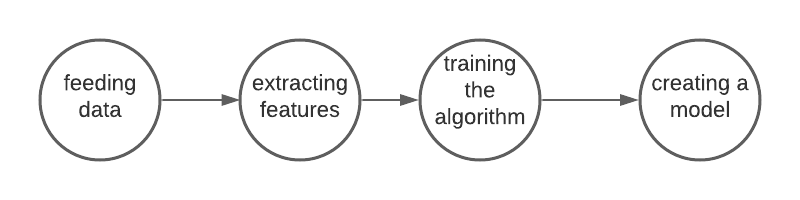
\includegraphics[width=5in]{bb.png}
            \caption{simple modeling}
            \label{fig:galaxy}
        \end{figure}
        \item a)We detect the fraudulent transactions from the Banksim dataset. This synthetically generated dataset consists of payments from various customers made in different periods and with different amounts.
        \pagebreak
        
        \textbf{Data preprocessing:}
           \begin{figure}[htp]
            \centering
                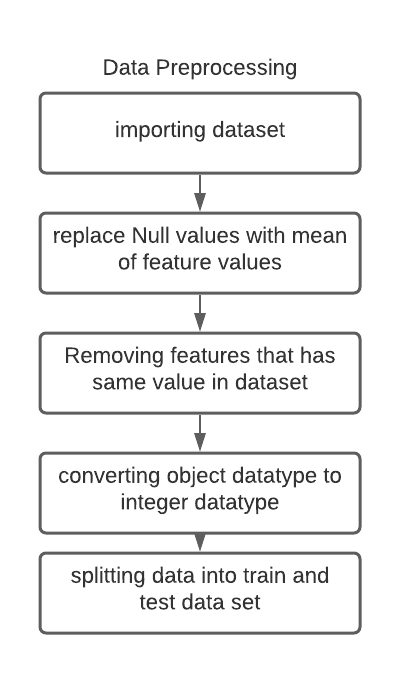
\includegraphics[height=5in]{preprocessing.png}
            \caption{Data preprocessing}
            \label{fig:gal}
        \end{figure}
        
        
         
        
        After the preprocessing, a model with logistic regression is imposed on the dataset.The models are trained and tested and we
        determine the model efficiency on the basis of accuracy.\\
        \\
        The architecture of these models is stated in the flowchart that follows
 
    \begin{figure}[htp]
    \centering
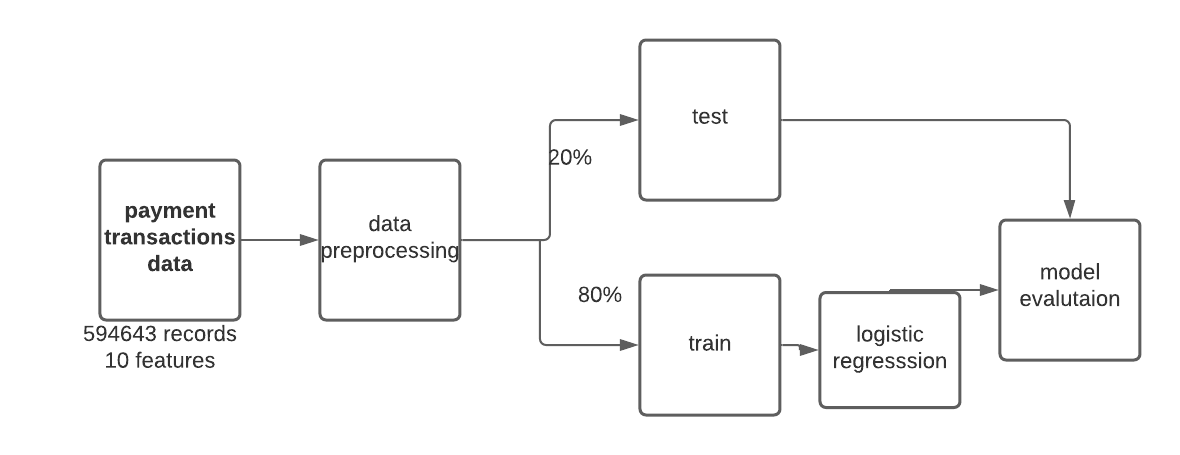
\includegraphics[height=2.5in]{diagram png.png}
\caption{system architecture}
    \label{fig:gal}
\end{figure}
   
   

At last, a baseline binary classification model using Logistic Regression is developed. The
accuracies are evaluated and compared to determine the model with the best possible
accuracy.
\pagebreak
   
\subsection{SETUP AND TOOLS}
    \begin{itemize}
            \item Operating System: Windows 10
            \item Required Software
             \begin{itemize}
                 \item Python 3.0
                 \item Google Collaboratory: An Online Python IDE for Machine Learning
                 \item Creately: A website providing tools to build the System Architecture and other related 
                 \item Lucidchart: A website providing tools to build Gantt Chart
                                designs     
             \end{itemize}
     \item REQUIRED LIBRARIES:
            \begin{itemize}
                           \item Python 
                        \item Numpy \item Pandas  \item Seaborn  
                         \item Sklearn\item CPU or GPU(recommended)
                        \end{itemize}
                        
    \end{itemize}
 
  \pagebreak
\section{CHAPTER 3}


\subsection{DATA ANALYSIS}

 	Importing the dataset, The data is  fetched  using a python library named pandas which consists of over 59000 records
   \textbf{ Importing data set:}data is converted into the tabular form using a pandas data frame
   \\
   \bigskip
\textbf{Search for Null values:}There may a chance of empty values in the given data set, so we need to fetch the indexes of the null value and replace them with the mean of feature values;
From the above output, the dataset has zero Null  values
\textbf{strength between each of feature}\\
In the given dataset, we need find the strength between each and 
every feature,i.e proportionality rate between them.

           \begin{figure}[htp]
    \centering
                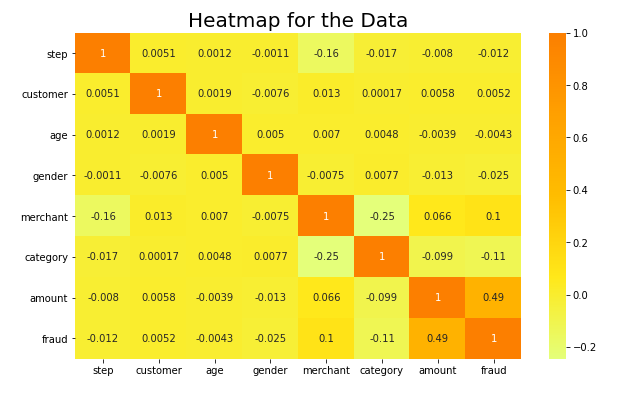
\includegraphics[height=4in]{i12.png}
    \caption{heatmap}
    \label{fig:galaxy}
\end{figure}


With the above heatmap:
\item 1) feature itself has proportionality constant=1,which is not useful for prediction
\item 2) the map value with second max value results in the most dependent feature



\pagebreak
\textbf{counting no of fraud data in Dataset}
          \begin{figure}[htp]
    \centering
                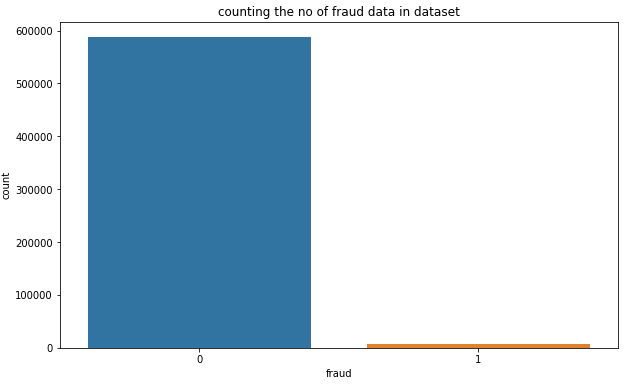
\includegraphics[height=4in]{i13.png}

    \caption{count of fraud data}
    \label{fig:galaxy}
\end{figure}
\pagebreak
\textbf{Grouped by category:}
Our hypothes is for fraudsters choosing the categories which people spend more.
 \begin{figure}[htp]
    \centering
                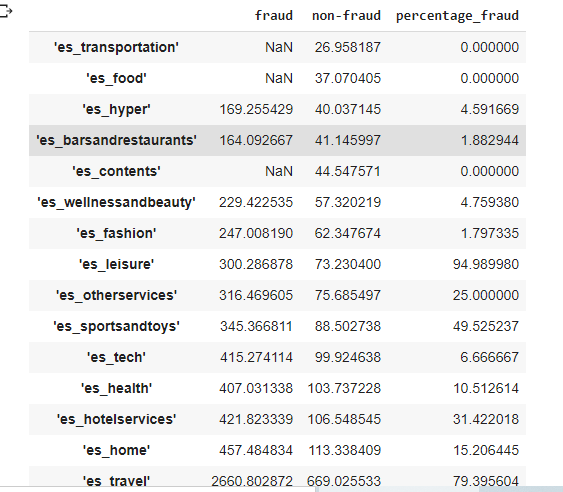
\includegraphics[height=5in]{i3.png}

    \caption{fraud vs non-fraud}
    \label{fig:galaxy}
\end{figure}
\\
 but as we can see in the table above we can say confidently say that a fraudulent transaction will be much more (about four times or more) than average for that category.
 \item Average amount spend it categories are similar; between 0-500 discarding the outliers, except for the travel category which goes very high
\newpage
\textbf{Fraudulent vs non-fraudulent Dataset:}
Again we can see in the histogram below that the fraudulent transactions are less in the count but more in amount.

          
           \begin{figure}[htp]
    \centering
                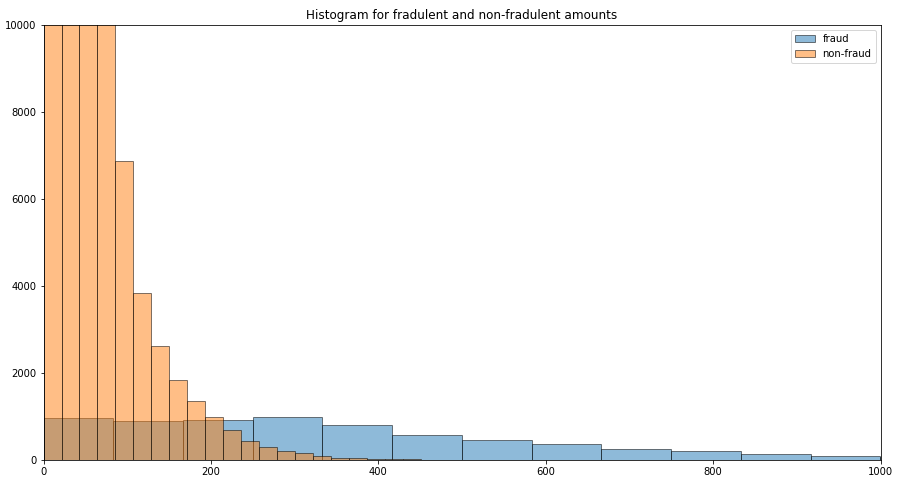
\includegraphics[height=4in]{i4.png}

    \caption{fraud vs non-fraud}
    \label{fig:galaxy}
\end{figure}

\newpage
\subsection{DATA PREPROCESSING}
  In this part we will preprocess the data and prepare for the training.\\
 
There are only one unique zipCode values so we will drop them
 \begin{figure}[htbp]
    \centering
    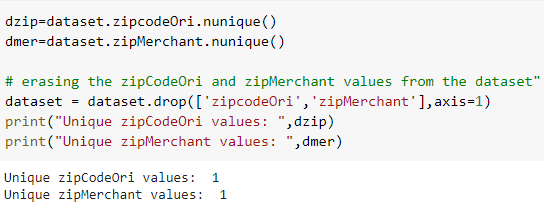
\includegraphics[height=2in]{i20.png}
    \caption{dropping features}
    \label{fig:galaxy}
\end{figure}
Here we will transform categorical features into numerical values. It is usually better to turn these type of categorical values into dummies because they have no relation in 
 \begin{figure}[htbp]
    \centering
    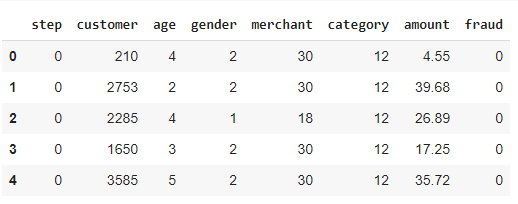
\includegraphics[height=2in]{i22.png}
    \caption{transforming features}
    \label{fig:galaxy}
\end{figure}
\\
\textbf{Undersampling Technique:}\\
Using  Undersampling Technique  for balancing the dataset. Resulted counts show that now we have exact number of class instances (1 and 0).Finally  ,
I will do a train test split for measuring the performance.
 \begin{figure}[htbp]
    \centering
    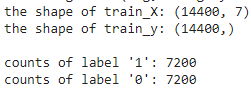
\includegraphics[height=1.5in]{i24.png}
    \caption{Undersampling }
    \label{fig:galaxy}
\end{figure}
\newline
\newline
\subsection{EXPERIMENTAL ANALYSIS AND RESULT:}
The performance metrics used to evaluate the models are the accuracy and the loss.
Our main aim was to increase the accuracy at the same time decrease the loss which means 
that the model is learning. \\
\textbf{Logistic Regression Algorithm:}
 \begin{figure}[htbp]
    \centering
    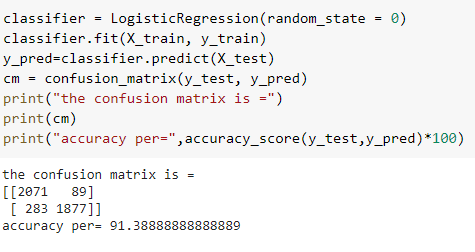
\includegraphics[height=2in]{i25.png}
        \caption{Logistic Regression }
    \label{fig:galaxy}
\end{figure}
\newpage
\textbf{K-Nearest Neighbor Algorithm:}
 \begin{figure}[htbp]
    \centering
    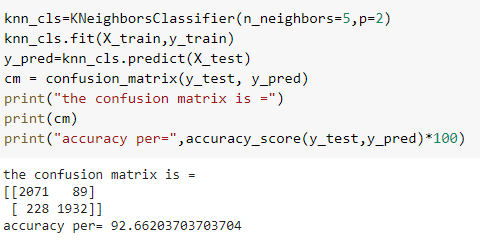
\includegraphics[height=2in]{i26.png}
    \caption{K-Nearest Neighbor}
    \label{fig:galaxy}
\end{figure}
\\
\textbf{Decision Tree Classification Algorithm:}
 \begin{figure}[htbp]
    \centering
    \includegraphics[height=1.5in]{i27.png}
    \caption{Decision Tree Classification}
    \label{fig:galaxy}
\end{figure}
\newpage
\textbf{Random Forest Algorithm:}
 \begin{figure}[htbp]
    \centering
    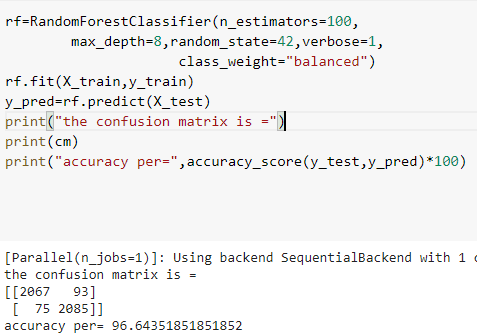
\includegraphics[width=3in,height=1.8in]{i28.png}
    \caption{Random Forest Algorithm}
    \label{fig:galaxy}
\end{figure}
\\
\textbf{Comparing Accuracies of the four Models:}
\begin{table}[htbp]
\begin{center}
\begin{tabular}{|p{5cm}|p{5cm}|}
\hline
MODEL&ACCURACY\\
\hline
Logistic Regression&91.38\\
\hline
K-Nearest Neighbor&92.66\\
\hline
Decision Tree Classification&96.11\\
\hline
Random Forest Algorithm&96.64\\
\hline
\end{tabular}
\end{center}
\caption{Accuracy matrix}
\end{table}
\pagebreak
\newpage
\section{CONCLUSION}
\subsection{ ADVANTAGES}: 
\begin{itemize}
    \item finding hidden and implicit correlations in the data
    \item automatic detection of possible fraud scenarios
    \item reduced number of verification measures
    \item real-time processing
\end{itemize}

\subsection{LIMITATIONS}  The amount of time required for the result and the cost for manual testing
and the limited availability of test kits. 
So we need a technique that provides the work faster and reduces the cost to check. Still, this model can return good accuracy and can be further improved.




\subsection{FUTURE SCOPE}
The findings obtained here are not in a generalized form that can be directly used in the global fraud detection problem. Here, we have considered a sample data set. As future work, some effective algorithms could be developed for the classification problem with variable misclassification costs.\\
 And the collection of more payment data will improve the model's accuracy.


 






\newpage
\section{REFERENCES}
\bibliographystyle{plain}
\cite{r1}.\cite{r2},\cite{r3},\cite{r4},\cite{r5},\cite{r6}

\bibliography{bbb.bib}

\end{document}
